% qkernel-hep report. Build:  cd report && pdflatex main && bibtex main && pdflatex main && pdflatex main
% Every result number is a \V{key} macro defined in numbers.tex, generated from results/ by
% scripts/report_numbers.py. Figures are generated from results/ by scripts/make_figures.py.
\documentclass[10pt,a4paper]{article}
\usepackage[T1]{fontenc}
\usepackage[utf8]{inputenc}
\usepackage{lmodern}
\usepackage{microtype}
\usepackage{amsmath,amssymb}
\usepackage{graphicx}
\usepackage{booktabs}
\usepackage[margin=2.1cm]{geometry}
\usepackage[font=small,labelfont=bf]{caption}
\usepackage[numbers,sort&compress]{natbib}
\usepackage{xcolor}
\usepackage[colorlinks=true,linkcolor=blue!50!black,citecolor=blue!50!black,urlcolor=blue!50!black]{hyperref}
\graphicspath{{../results/figures/notitle/}}
% Generated by scripts/report_numbers.py from results/ -- do not edit by hand.
\makeatletter
\newcommand{\defval}[2]{\expandafter\def\csname qk@#1\endcsname{#2}}
\newcommand{\V}[1]{\ifcsname qk@#1\endcsname\csname qk@#1\endcsname\else\PackageError{numbers}{Undefined value #1}{}\fi}
\makeatother
\defval{data_rows}{\ensuremath{818{,}238}}% data_summary.json n_rows
\defval{data_signal}{\ensuremath{279{,}560}}% data_summary.json n_signal
\defval{data_background}{\ensuremath{538{,}678}}% data_summary.json n_background
\defval{data_raw_features}{\ensuremath{30}}% data_summary.json n_features_raw
\defval{data_features}{\ensuremath{19}}% data_summary.json n_selected_features
\defval{ntrain}{\ensuremath{500}}% main_grid/meta.json config.n_train
\defval{ntest}{\ensuremath{1{,}000}}% main_grid/meta.json config.n_test
\defval{nseeds}{\ensuremath{5}}% main_grid/meta.json config.seeds
\defval{qubits_main_min}{\ensuremath{2}}% main_grid/meta.json config.qubits
\defval{qubits_main_max}{\ensuremath{10}}% main_grid/meta.json config.qubits
\defval{qubits_main}{\ensuremath{2, 4, 6, 8, 10}}% main_grid/meta.json config.qubits
\defval{qubits_big}{\ensuremath{12, 14}}% big_qubits/meta.json config.qubits
\defval{qubits_big_max}{\ensuremath{14}}% big_qubits/meta.json config.qubits
\defval{bandwidths}{\ensuremath{0.05, 0.1, 0.25, 0.5, 1}}% main_grid/meta.json config.bandwidths
\defval{bw_min}{\ensuremath{0.05}}% main_grid/meta.json config.bandwidths
\defval{bw_max}{\ensuremath{1}}% main_grid/meta.json config.bandwidths
\defval{bandwidths_big}{\ensuremath{0.1, 1}}% big_qubits/meta.json config.bandwidths
\defval{lambdas}{\ensuremath{0.001, 0.01, 0.1}}% main_grid/meta.json config.lambdas
\defval{sweep_ntrain}{\ensuremath{100, 250, 500, 1000}}% n_sweep/meta.json config.n_train
\defval{sweep_qubits}{\ensuremath{4, 8}}% n_sweep/meta.json config.qubits
\defval{fs_qubits}{\ensuremath{4, 8}}% fs_gbdt/meta.json config.qubits
\defval{rows_main}{\ensuremath{375}}% main_grid/runs.jsonl line count
\defval{rows_big}{\ensuremath{20}}% big_qubits/runs.jsonl line count
\defval{rows_main_big}{\ensuremath{395}}% main_grid + big_qubits runs.jsonl
\defval{rows_sweep}{\ensuremath{80}}% n_sweep/runs.jsonl line count
\defval{rows_fs}{\ensuremath{150}}% fs_gbdt/runs.jsonl line count
\defval{nconfigs}{\ensuremath{79}}% h2_analysis.json H2.n_configs
\defval{nboot}{\ensuremath{2{,}000}}% h2_analysis.json bootstrap_resamples
\defval{h1_fid_cb}{\ensuremath{58}}% h2_analysis.json H1.fidelity.vs_best_classical
\defval{h1_fid_ns}{\ensuremath{21}}% h2_analysis.json H1.fidelity.vs_best_classical
\defval{h1_fid_qb}{\ensuremath{0}}% h2_analysis.json H1.fidelity.vs_best_classical
\defval{h1_fid_maxgap}{\ensuremath{+0.0033}}% h2_analysis.json H1.fidelity.max_gap_vs_best
\defval{h1_pqk_cb}{\ensuremath{60}}% h2_analysis.json H1.projected.vs_best_classical
\defval{h1_pqk_ns}{\ensuremath{19}}% h2_analysis.json H1.projected.vs_best_classical
\defval{h1_pqk_qb}{\ensuremath{0}}% h2_analysis.json H1.projected.vs_best_classical
\defval{h1_pqk_maxgap}{\ensuremath{+0.0019}}% h2_analysis.json H1.projected.max_gap_vs_best
\defval{h1_chance}{\ensuremath{3.6}}% h2_analysis.json H1.chance_positive_hits_expected_per_kernel
\defval{h1_rbf_hits}{\ensuremath{2}}% summary_table.csv rows with gap_vs_rbf_label or pqk_gap_vs_rbf_label == quantum better
\defval{h1_rbf0_desc}{ZZ, reps~1, $n=2$, $c=0.1$}% summary_table.csv
\defval{h1_rbf0_gap}{\ensuremath{+0.0071} $\pm$ \ensuremath{0.0058}}% summary_table.csv gap_vs_rbf, gap_vs_rbf_sd
\defval{h1_rbf0_best}{\ensuremath{+0.0017}}% summary_table.csv gap_vs_best
\defval{h1_rbf1_desc}{ZZ, reps~2, $n=2$, $c=0.05$}% summary_table.csv
\defval{h1_rbf1_gap}{\ensuremath{+0.0073} $\pm$ \ensuremath{0.0038}}% summary_table.csv gap_vs_rbf, gap_vs_rbf_sd
\defval{h1_rbf1_best}{\ensuremath{+0.0018}}% summary_table.csv gap_vs_best
\defval{best_cl_n2}{\ensuremath{0.737}}% summary_table.csv best_classical_auc, main_grid n=2
\defval{best_cl_n10}{\ensuremath{0.822}}% summary_table.csv best_classical_auc, main_grid n=10
\defval{cv_z_n10_auc}{\ensuremath{0.817}}% h2_analysis.json H1.cv_selected_bandwidth
\defval{cv_z_n10_gap}{\ensuremath{-0.0051}}% h2_analysis.json H1.cv_selected_bandwidth
\defval{cv_zz2_n10_gap}{\ensuremath{-0.028}}% h2_analysis.json H1.cv_selected_bandwidth
\defval{cv_zz2_n14_auc}{\ensuremath{0.751}}% h2_analysis.json H1.cv_selected_bandwidth
\defval{cv_zz2_n14_gap}{\ensuremath{-0.071}}% h2_analysis.json H1.cv_selected_bandwidth
\defval{cv_zz_first_behind}{\ensuremath{6}}% h2_analysis.json H1.cv_selected_bandwidth (smallest n with ZZ classical better)
\defval{h2_pool_l0}{\ensuremath{-0.50}~[\ensuremath{-0.65}, \ensuremath{-0.32}]}% h2_analysis.json H2.pooled.lambda=0
\defval{h2_part_l0}{\ensuremath{-0.72}~[\ensuremath{-0.82}, \ensuremath{-0.59}]}% h2_analysis.json H2.partial_controlling_log_var.lambda=0
\defval{h2_within_l0_z}{\ensuremath{-0.62}~[\ensuremath{-0.86}, \ensuremath{-0.29}]}% h2_analysis.json H2.within_feature_map.lambda=0
\defval{h2_wpart_l0_z}{\ensuremath{-0.82}~[\ensuremath{-0.92}, \ensuremath{-0.59}]}% h2_analysis.json H2.within_feature_map_partial.lambda=0
\defval{h2_within_l0_zza}{\ensuremath{-0.37}~[\ensuremath{-0.65}, \ensuremath{-0.01}]}% h2_analysis.json H2.within_feature_map.lambda=0
\defval{h2_wpart_l0_zza}{\ensuremath{-0.62}~[\ensuremath{-0.81}, \ensuremath{-0.27}]}% h2_analysis.json H2.within_feature_map_partial.lambda=0
\defval{h2_within_l0_zzb}{\ensuremath{-0.25}~[\ensuremath{-0.55}, \ensuremath{+0.12}]}% h2_analysis.json H2.within_feature_map.lambda=0
\defval{h2_wpart_l0_zzb}{\ensuremath{-0.66}~[\ensuremath{-0.84}, \ensuremath{-0.28}]}% h2_analysis.json H2.within_feature_map_partial.lambda=0
\defval{h2_pool_l0001}{\ensuremath{-0.63}~[\ensuremath{-0.74}, \ensuremath{-0.46}]}% h2_analysis.json H2.pooled.lambda=0.001
\defval{h2_part_l0001}{\ensuremath{-0.77}~[\ensuremath{-0.84}, \ensuremath{-0.67}]}% h2_analysis.json H2.partial_controlling_log_var.lambda=0.001
\defval{h2_within_l0001_z}{\ensuremath{-0.79}~[\ensuremath{-0.92}, \ensuremath{-0.57}]}% h2_analysis.json H2.within_feature_map.lambda=0.001
\defval{h2_wpart_l0001_z}{\ensuremath{-0.89}~[\ensuremath{-0.95}, \ensuremath{-0.70}]}% h2_analysis.json H2.within_feature_map_partial.lambda=0.001
\defval{h2_within_l0001_zza}{\ensuremath{-0.43}~[\ensuremath{-0.69}, \ensuremath{-0.01}]}% h2_analysis.json H2.within_feature_map.lambda=0.001
\defval{h2_wpart_l0001_zza}{\ensuremath{-0.59}~[\ensuremath{-0.77}, \ensuremath{-0.28}]}% h2_analysis.json H2.within_feature_map_partial.lambda=0.001
\defval{h2_within_l0001_zzb}{\ensuremath{-0.37}~[\ensuremath{-0.66}, \ensuremath{+0.06}]}% h2_analysis.json H2.within_feature_map.lambda=0.001
\defval{h2_wpart_l0001_zzb}{\ensuremath{-0.66}~[\ensuremath{-0.82}, \ensuremath{-0.38}]}% h2_analysis.json H2.within_feature_map_partial.lambda=0.001
\defval{h2_pool_l001}{\ensuremath{-0.44}~[\ensuremath{-0.61}, \ensuremath{-0.22}]}% h2_analysis.json H2.pooled.lambda=0.01
\defval{h2_part_l001}{\ensuremath{-0.66}~[\ensuremath{-0.75}, \ensuremath{-0.54}]}% h2_analysis.json H2.partial_controlling_log_var.lambda=0.01
\defval{h2_within_l001_z}{\ensuremath{-0.77}~[\ensuremath{-0.90}, \ensuremath{-0.56}]}% h2_analysis.json H2.within_feature_map.lambda=0.01
\defval{h2_wpart_l001_z}{\ensuremath{-0.84}~[\ensuremath{-0.93}, \ensuremath{-0.62}]}% h2_analysis.json H2.within_feature_map_partial.lambda=0.01
\defval{h2_within_l001_zza}{\ensuremath{-0.27}~[\ensuremath{-0.66}, \ensuremath{+0.21}]}% h2_analysis.json H2.within_feature_map.lambda=0.01
\defval{h2_wpart_l001_zza}{\ensuremath{-0.49}~[\ensuremath{-0.73}, \ensuremath{-0.14}]}% h2_analysis.json H2.within_feature_map_partial.lambda=0.01
\defval{h2_within_l001_zzb}{\ensuremath{-0.06}~[\ensuremath{-0.45}, \ensuremath{+0.40}]}% h2_analysis.json H2.within_feature_map.lambda=0.01
\defval{h2_wpart_l001_zzb}{\ensuremath{-0.61}~[\ensuremath{-0.79}, \ensuremath{-0.34}]}% h2_analysis.json H2.within_feature_map_partial.lambda=0.01
\defval{h2_pool_l01}{\ensuremath{+0.34}~[\ensuremath{+0.09}, \ensuremath{+0.54}]}% h2_analysis.json H2.pooled.lambda=0.1
\defval{h2_part_l01}{\ensuremath{+0.03}~[\ensuremath{-0.19}, \ensuremath{+0.25}]}% h2_analysis.json H2.partial_controlling_log_var.lambda=0.1
\defval{h2_within_l01_z}{\ensuremath{-0.49}~[\ensuremath{-0.77}, \ensuremath{-0.10}]}% h2_analysis.json H2.within_feature_map.lambda=0.1
\defval{h2_wpart_l01_z}{\ensuremath{-0.48}~[\ensuremath{-0.77}, \ensuremath{-0.08}]}% h2_analysis.json H2.within_feature_map_partial.lambda=0.1
\defval{h2_within_l01_zza}{\ensuremath{+0.50}~[\ensuremath{+0.07}, \ensuremath{+0.78}]}% h2_analysis.json H2.within_feature_map.lambda=0.1
\defval{h2_wpart_l01_zza}{\ensuremath{-0.31}~[\ensuremath{-0.56}, \ensuremath{+0.15}]}% h2_analysis.json H2.within_feature_map_partial.lambda=0.1
\defval{h2_within_l01_zzb}{\ensuremath{+0.59}~[\ensuremath{+0.23}, \ensuremath{+0.81}]}% h2_analysis.json H2.within_feature_map.lambda=0.1
\defval{h2_wpart_l01_zzb}{\ensuremath{-0.40}~[\ensuremath{-0.61}, \ensuremath{-0.05}]}% h2_analysis.json H2.within_feature_map_partial.lambda=0.1
\defval{h2_logvar}{\ensuremath{+0.51}~[\ensuremath{+0.30}, \ensuremath{+0.68}]}% h2_analysis.json H2.pooled.log_kernel_variance
\defval{h2_ratio_pool}{\ensuremath{-0.63}~[\ensuremath{-0.75}, \ensuremath{-0.48}]}% h2_analysis.json H2.label_aware.pooled
\defval{h2_ratio_part}{\ensuremath{-0.61}~[\ensuremath{-0.73}, \ensuremath{-0.44}]}% h2_analysis.json H2.label_aware.partial_controlling_log_var
\defval{h2_sc_min}{\ensuremath{4.4}}% h2_analysis.json H2.label_aware.bound_regime.s_classical_min
\defval{h2_sq_auc}{\ensuremath{+0.80}~[\ensuremath{+0.70}, \ensuremath{+0.86}]}% h2_analysis.json H2.label_aware.bound_regime
\defval{sqrtN}{\ensuremath{22.4}}% h2_analysis.json H2.huang_necessary_condition.sqrt_N
\defval{nc_max_l0}{\ensuremath{3.4\times10^{5}}}% h2_analysis.json H2.huang_necessary_condition.by_lambda.lambda=0.max_g
\defval{nc_above_l0}{\ensuremath{61}}% h2_analysis.json H2.huang_necessary_condition.by_lambda.lambda=0.n_above_sqrt_N
\defval{nc_above_l0_cb}{\ensuremath{50}}% ... lambda=0.gap_labels_above
\defval{nc_above_l0_ns}{\ensuremath{11}}% ... lambda=0.gap_labels_above
\defval{nc_max_l0001}{\ensuremath{49.7}}% h2_analysis.json H2.huang_necessary_condition.by_lambda.lambda=0.001.max_g
\defval{nc_above_l0001}{\ensuremath{17}}% h2_analysis.json H2.huang_necessary_condition.by_lambda.lambda=0.001.n_above_sqrt_N
\defval{nc_above_l0001_cb}{\ensuremath{16}}% ... lambda=0.001.gap_labels_above
\defval{nc_above_l0001_ns}{\ensuremath{1}}% ... lambda=0.001.gap_labels_above
\defval{nc_max_l001}{\ensuremath{19.6}}% h2_analysis.json H2.huang_necessary_condition.by_lambda.lambda=0.01.max_g
\defval{nc_above_l001}{\ensuremath{0}}% h2_analysis.json H2.huang_necessary_condition.by_lambda.lambda=0.01.n_above_sqrt_N
\defval{nc_above_l001_cb}{\ensuremath{0}}% ... lambda=0.01.gap_labels_above
\defval{nc_above_l001_ns}{\ensuremath{0}}% ... lambda=0.01.gap_labels_above
\defval{nc_max_l01}{\ensuremath{7.4}}% h2_analysis.json H2.huang_necessary_condition.by_lambda.lambda=0.1.max_g
\defval{nc_above_l01}{\ensuremath{0}}% h2_analysis.json H2.huang_necessary_condition.by_lambda.lambda=0.1.n_above_sqrt_N
\defval{nc_above_l01_cb}{\ensuremath{0}}% ... lambda=0.1.gap_labels_above
\defval{nc_above_l01_ns}{\ensuremath{0}}% ... lambda=0.1.gap_labels_above
\defval{h3_cells}{\ensuremath{15}}% h2_analysis.json H3.trend_vs_qubits
\defval{h3_held}{\ensuremath{4}}% h2_analysis.json H3.trend_vs_qubits.H3_holds_here
\defval{h3_held_list}{ZZ, reps 1 $c=0.25$; ZZ, reps 1 $c=0.5$; ZZ, reps 1 $c=1$; ZZ, reps 2 $c=0.5$}% h2_analysis.json H3.trend_vs_qubits
\defval{h3_slope_min}{\ensuremath{0.27}}% h2_analysis.json H3.trend_vs_qubits (ZZ, c>=0.25)
\defval{h3_slope_max}{\ensuremath{0.49}}% h2_analysis.json H3.trend_vs_qubits (ZZ, c>=0.25)
\defval{h3_z_auc_rises}{\ensuremath{5}}% h2_analysis.json H3.trend_vs_qubits (Z map auc_trend)
\defval{h3_z_cells}{\ensuremath{5}}% h2_analysis.json H3.trend_vs_qubits (Z map)
\defval{h3_conc_n}{\ensuremath{17}}% h2_analysis.json H3.low_variance_regimes[concentrated]
\defval{h3_conc_med}{\ensuremath{0.550}}% h2_analysis.json H3.low_variance_regimes[concentrated]
\defval{h3_conc_max}{\ensuremath{0.720}}% h2_analysis.json H3.low_variance_regimes[concentrated]
\defval{h3_flat_n}{\ensuremath{5}}% h2_analysis.json H3.low_variance_regimes[near-constant]
\defval{h3_flat_med}{\ensuremath{0.782}}% h2_analysis.json H3.low_variance_regimes[near-constant]
\defval{h3_depth_cells}{\ensuremath{25}}% h2_analysis.json H3.depth_zz_reps2_vs_reps1
\defval{h3_depth_more_conc}{\ensuremath{12}}% h2_analysis.json H3.depth_zz_reps2_vs_reps1
\defval{h3_depth_auc_lower}{\ensuremath{14}}% h2_analysis.json H3.depth_zz_reps2_vs_reps1
\defval{h3_rho_var_auc}{\ensuremath{+0.40}~[\ensuremath{+0.18}, \ensuremath{+0.58}]}% h2_analysis.json H3.spearman_log_var_vs_qsvm_auc
\defval{ex_zz2_c1_var_n2}{\ensuremath{5.2\times10^{-2}}}% summary_table.csv zz2 c=1 n=2 q_offdiag_var
\defval{ex_zz2_c1_var_n14}{\ensuremath{7.4\times10^{-8}}}% summary_table.csv zz2 c=1 n=14 q_offdiag_var
\defval{ex_zz2_c1_auc_n2}{\ensuremath{0.546}}% summary_table.csv zz2 c=1 n=2 qsvm_auc
\defval{ex_zz2_c1_auc_n14}{\ensuremath{0.523}}% summary_table.csv zz2 c=1 n=14 qsvm_auc
\defval{h4_cells}{\ensuremath{15}}% h2_analysis.json H4.cells
\defval{h4_auc_rec}{\ensuremath{15}}% h2_analysis.json H4.cells.performance_recovered
\defval{h4_var_raised}{\ensuremath{8}}% h2_analysis.json H4.cells.concentration_reduced
\defval{h4_g01_mono}{\ensuremath{7}}% h2_analysis.json H4.cells.g_lam0.01_monotone_toward_1
\defval{h4_g01_small_min}{\ensuremath{2.1}}% h2_analysis.json H4.cells.g_lam0.01_small_c
\defval{h4_g01_small_max}{\ensuremath{4.7}}% h2_analysis.json H4.cells.g_lam0.01_small_c
\defval{h4_g01_argmax_zz}{\ensuremath{0.1, 0.25, 0.5}}% h2_analysis.json H4.cells.g_lam0.01_argmax_c (ZZ)
\defval{h4_g0_closer}{\ensuremath{15}}% h2_analysis.json H4.cells.g_lam0_closer_to_1_at_small_c
\defval{h4_g0_mono}{\ensuremath{15}}% h2_analysis.json H4.cells.g_lam0_monotone_toward_1
\defval{h4_g0_small_min}{\ensuremath{2.8}}% h2_analysis.json H4.cells.g_lam0_small_c
\defval{h4_g0_small_max}{\ensuremath{398}}% h2_analysis.json H4.cells.g_lam0_small_c
\defval{h4_g0_large_min}{\ensuremath{173}}% h2_analysis.json H4.cells.g_lam0_large_c
\defval{h4_g0_large_max}{\ensuremath{3.4\times10^{5}}}% h2_analysis.json H4.cells.g_lam0_large_c
\defval{ex_h4_auc_small}{\ensuremath{0.796}}% h2_analysis.json H4.cells (ZZ reps 2, n=8) auc_small
\defval{ex_h4_auc_large}{\ensuremath{0.511}}% h2_analysis.json H4.cells (ZZ reps 2, n=8) auc_large
\defval{ex_h4_dvar}{\ensuremath{2.8}}% h2_analysis.json H4.cells (ZZ reps 2, n=8) dlog10_var
\defval{ex_h4_g01_small}{\ensuremath{3.6}}% h2_analysis.json H4.cells (ZZ reps 2, n=8)
\defval{ex_h4_g01_large}{\ensuremath{5.5}}% h2_analysis.json H4.cells (ZZ reps 2, n=8)
\defval{ex_h4_g01_argmax}{\ensuremath{0.10}}% h2_analysis.json H4.cells (ZZ reps 2, n=8)
\defval{rob_unchanged}{\ensuremath{4}}% h2_analysis.json robustness.verdict_comparison
\defval{rob_bc_pca_n4}{\ensuremath{0.788}}% h2_analysis.json robustness.classical_auc.pca.n4
\defval{rob_gbdt_pca_n4}{\ensuremath{0.784}}% h2_analysis.json robustness.classical_auc.pca.n4
\defval{rob_rbf_pca_n4}{\ensuremath{0.787}}% h2_analysis.json robustness.classical_auc.pca.n4
\defval{rob_bc_pca_n8}{\ensuremath{0.817}}% h2_analysis.json robustness.classical_auc.pca.n8
\defval{rob_gbdt_pca_n8}{\ensuremath{0.803}}% h2_analysis.json robustness.classical_auc.pca.n8
\defval{rob_rbf_pca_n8}{\ensuremath{0.815}}% h2_analysis.json robustness.classical_auc.pca.n8
\defval{rob_bc_fs_n4}{\ensuremath{0.825}}% h2_analysis.json robustness.classical_auc.feature_selection.n4
\defval{rob_gbdt_fs_n4}{\ensuremath{0.822}}% h2_analysis.json robustness.classical_auc.feature_selection.n4
\defval{rob_rbf_fs_n4}{\ensuremath{0.812}}% h2_analysis.json robustness.classical_auc.feature_selection.n4
\defval{rob_bc_fs_n8}{\ensuremath{0.831}}% h2_analysis.json robustness.classical_auc.feature_selection.n8
\defval{rob_gbdt_fs_n8}{\ensuremath{0.830}}% h2_analysis.json robustness.classical_auc.feature_selection.n8
\defval{rob_rbf_fs_n8}{\ensuremath{0.816}}% h2_analysis.json robustness.classical_auc.feature_selection.n8
\defval{rob_dq}{\ensuremath{+0.028}}% h2_analysis.json robustness.median_change_fs_minus_pca.qsvm_auc
\defval{rob_dbc}{\ensuremath{+0.026}}% h2_analysis.json robustness.median_change_fs_minus_pca.best_classical_auc
\defval{rob_dvar}{\ensuremath{+0.10}}% h2_analysis.json robustness.median_change_fs_minus_pca.log10_var
\defval{rob_bias}{\ensuremath{0.0016}}% h2_analysis.json robustness.best_of_three_test_auc_bias
\defval{rob_pca_nconf}{\ensuremath{30}}% h2_analysis.json robustness.pca.H1.n_configs
\defval{rob_pca_fid_qb}{\ensuremath{0}}% h2_analysis.json robustness.pca.H1.fidelity
\defval{rob_pca_pqk_qb}{\ensuremath{0}}% h2_analysis.json robustness.pca.H1.projected
\defval{rob_pca_h2_l0}{\ensuremath{-0.71}~[\ensuremath{-0.86}, \ensuremath{-0.49}]}% h2_analysis.json robustness.pca.H2.pooled.lambda=0
\defval{rob_pca_h2part_l0}{\ensuremath{-0.82}~[\ensuremath{-0.92}, \ensuremath{-0.62}]}% h2_analysis.json robustness.pca.H2.partial.lambda=0
\defval{rob_pca_h2_l0001}{\ensuremath{-0.71}~[\ensuremath{-0.84}, \ensuremath{-0.47}]}% h2_analysis.json robustness.pca.H2.pooled.lambda=0.001
\defval{rob_pca_h2part_l0001}{\ensuremath{-0.78}~[\ensuremath{-0.89}, \ensuremath{-0.59}]}% h2_analysis.json robustness.pca.H2.partial.lambda=0.001
\defval{rob_pca_h2_l001}{\ensuremath{-0.62}~[\ensuremath{-0.81}, \ensuremath{-0.30}]}% h2_analysis.json robustness.pca.H2.pooled.lambda=0.01
\defval{rob_pca_h2part_l001}{\ensuremath{-0.72}~[\ensuremath{-0.85}, \ensuremath{-0.50}]}% h2_analysis.json robustness.pca.H2.partial.lambda=0.01
\defval{rob_pca_h2_l01}{\ensuremath{+0.21}~[\ensuremath{-0.24}, \ensuremath{+0.56}]}% h2_analysis.json robustness.pca.H2.pooled.lambda=0.1
\defval{rob_pca_h2part_l01}{\ensuremath{+0.03}~[\ensuremath{-0.35}, \ensuremath{+0.36}]}% h2_analysis.json robustness.pca.H2.partial.lambda=0.1
\defval{rob_pca_h3_held}{\ensuremath{1}}% h2_analysis.json robustness.pca.H3
\defval{rob_pca_h3_cells}{\ensuremath{15}}% h2_analysis.json robustness.pca.H3
\defval{rob_pca_h4_cells}{\ensuremath{6}}% h2_analysis.json robustness.pca.H4
\defval{rob_pca_h4_auc}{\ensuremath{6}}% h2_analysis.json robustness.pca.H4
\defval{rob_pca_h4_var}{\ensuremath{4}}% h2_analysis.json robustness.pca.H4
\defval{rob_pca_h4_g}{\ensuremath{2}}% h2_analysis.json robustness.pca.H4
\defval{rob_fs_nconf}{\ensuremath{30}}% h2_analysis.json robustness.feature_selection.H1.n_configs
\defval{rob_fs_fid_qb}{\ensuremath{0}}% h2_analysis.json robustness.feature_selection.H1.fidelity
\defval{rob_fs_fid_cv_qb}{\ensuremath{0}}% h2_analysis.json robustness.feature_selection.H1.fidelity.vs_cv_selected_classical
\defval{rob_fs_pqk_qb}{\ensuremath{0}}% h2_analysis.json robustness.feature_selection.H1.projected
\defval{rob_fs_pqk_cv_qb}{\ensuremath{0}}% h2_analysis.json robustness.feature_selection.H1.projected.vs_cv_selected_classical
\defval{rob_fs_h2_l0}{\ensuremath{-0.73}~[\ensuremath{-0.84}, \ensuremath{-0.54}]}% h2_analysis.json robustness.feature_selection.H2.pooled.lambda=0
\defval{rob_fs_h2part_l0}{\ensuremath{-0.87}~[\ensuremath{-0.94}, \ensuremath{-0.66}]}% h2_analysis.json robustness.feature_selection.H2.partial.lambda=0
\defval{rob_fs_h2_l0001}{\ensuremath{-0.41}~[\ensuremath{-0.64}, \ensuremath{-0.07}]}% h2_analysis.json robustness.feature_selection.H2.pooled.lambda=0.001
\defval{rob_fs_h2part_l0001}{\ensuremath{-0.75}~[\ensuremath{-0.88}, \ensuremath{-0.46}]}% h2_analysis.json robustness.feature_selection.H2.partial.lambda=0.001
\defval{rob_fs_h2_l001}{\ensuremath{-0.16}~[\ensuremath{-0.46}, \ensuremath{+0.21}]}% h2_analysis.json robustness.feature_selection.H2.pooled.lambda=0.01
\defval{rob_fs_h2part_l001}{\ensuremath{-0.65}~[\ensuremath{-0.82}, \ensuremath{-0.31}]}% h2_analysis.json robustness.feature_selection.H2.partial.lambda=0.01
\defval{rob_fs_h2_l01}{\ensuremath{+0.42}~[\ensuremath{+0.03}, \ensuremath{+0.69}]}% h2_analysis.json robustness.feature_selection.H2.pooled.lambda=0.1
\defval{rob_fs_h2part_l01}{\ensuremath{-0.16}~[\ensuremath{-0.47}, \ensuremath{+0.24}]}% h2_analysis.json robustness.feature_selection.H2.partial.lambda=0.1
\defval{rob_fs_h3_held}{\ensuremath{2}}% h2_analysis.json robustness.feature_selection.H3
\defval{rob_fs_h3_cells}{\ensuremath{15}}% h2_analysis.json robustness.feature_selection.H3
\defval{rob_fs_h4_cells}{\ensuremath{6}}% h2_analysis.json robustness.feature_selection.H4
\defval{rob_fs_h4_auc}{\ensuremath{6}}% h2_analysis.json robustness.feature_selection.H4
\defval{rob_fs_h4_var}{\ensuremath{4}}% h2_analysis.json robustness.feature_selection.H4
\defval{rob_fs_h4_g}{\ensuremath{2}}% h2_analysis.json robustness.feature_selection.H4
\defval{ang_pca_n4}{\ensuremath{1.26}}% h2_analysis.json robustness.angle_spread.pca_n4
\defval{ang_pca_n8}{\ensuremath{1.01}}% h2_analysis.json robustness.angle_spread.pca_n8
\defval{ang_fs_n4}{\ensuremath{1.31}}% h2_analysis.json robustness.angle_spread.gbdt_importance_n4
\defval{ang_fs_n8}{\ensuremath{1.52}}% h2_analysis.json robustness.angle_spread.gbdt_importance_n8
\defval{rob_top2}{\texttt{DER\_mass\_transverse\_met\_lep} and \texttt{DER\_mass\_vis}}% h2_analysis.json robustness.selected_features (first two in every seed and n)
\defval{nz_shots}{\ensuremath{100, 1000, 10000}}% noise.csv shots
\defval{nz_p}{\ensuremath{0.01, 0.05, 0.1}}% noise.csv p_tot
\defval{nz_c_healthy}{\ensuremath{0.1}}% noise.csv bandwidth (healthy)
\defval{nz_c_conc}{\ensuremath{1.0}}% noise.csv bandwidth (concentrated)
\defval{nz_h4_ex}{\ensuremath{0.779}}% noise.csv mean qsvm_auc n4_healthy shots=exact p=0
\defval{nz_h4_10k}{\ensuremath{0.768}}% noise.csv mean qsvm_auc n4_healthy shots=10000 p=0
\defval{nz_h4_1k}{\ensuremath{0.748}}% noise.csv mean qsvm_auc n4_healthy shots=1000 p=0
\defval{nz_h4_100}{\ensuremath{0.706}}% noise.csv mean qsvm_auc n4_healthy shots=100 p=0
\defval{nz_h4_ex_p01}{\ensuremath{0.786}}% noise.csv mean qsvm_auc n4_healthy exact p=0.1
\defval{nz_h4_100_p01}{\ensuremath{0.717}}% noise.csv mean qsvm_auc n4_healthy 100 shots p=0.1
\defval{nz_h8_ex}{\ensuremath{0.770}}% noise.csv mean qsvm_auc n8_healthy shots=exact p=0
\defval{nz_h8_10k}{\ensuremath{0.769}}% noise.csv mean qsvm_auc n8_healthy shots=10000 p=0
\defval{nz_h8_1k}{\ensuremath{0.768}}% noise.csv mean qsvm_auc n8_healthy shots=1000 p=0
\defval{nz_h8_100}{\ensuremath{0.747}}% noise.csv mean qsvm_auc n8_healthy shots=100 p=0
\defval{nz_h8_ex_p01}{\ensuremath{0.770}}% noise.csv mean qsvm_auc n8_healthy exact p=0.1
\defval{nz_h8_100_p01}{\ensuremath{0.748}}% noise.csv mean qsvm_auc n8_healthy 100 shots p=0.1
\defval{nz_conc_min}{\ensuremath{0.503}}% noise.csv mean qsvm_auc, concentrated configs, all conditions
\defval{nz_conc_max}{\ensuremath{0.524}}% noise.csv mean qsvm_auc, concentrated configs, all conditions
\defval{nz_bc4}{\ensuremath{0.788}}% noise.csv mean best_classical_auc n4_healthy
\defval{nz_bc8}{\ensuremath{0.817}}% noise.csv mean best_classical_auc n8_healthy
\defval{nz_var8c_ex}{\ensuremath{8.18\times10^{-5}}}% noise.csv mean offdiag_var n8_concentrated exact p=0
\defval{nz_var8c_100}{\ensuremath{1.35\times10^{-4}}}% noise.csv mean offdiag_var n8_concentrated 100 shots p=0
\defval{hw_backend}{\texttt{ibm\_marrakesh}}% real_ibm_marrakesh_20261110_003008.json backend
\defval{hw_n}{\ensuremath{4}}% real_ibm_marrakesh_20261110_003008.json config.n
\defval{hw_reps}{\ensuremath{1}}% real_ibm_marrakesh_20261110_003008.json config.reps
\defval{hw_c}{\ensuremath{0.05}}% real_ibm_marrakesh_20261110_003008.json config.c
\defval{hw_ntrain}{\ensuremath{24}}% real_ibm_marrakesh_20261110_003008.json config.ntrain
\defval{hw_ntest}{\ensuremath{24}}% real_ibm_marrakesh_20261110_003008.json config.ntest
\defval{hw_shots}{\ensuremath{500}}% real_ibm_marrakesh_20261110_003008.json config.shots
\defval{hw_circuits}{\ensuremath{996}}% real_ibm_marrakesh_20261110_003008.json n_circuits
\defval{hw_depth}{\ensuremath{41}}% real_ibm_marrakesh_20261110_003008.json mean_depth
\defval{hw_2q}{\ensuremath{9}}% real_ibm_marrakesh_20261110_003008.json mean_2q_gates
\defval{hw_qpu_s}{\ensuremath{143}}% real_ibm_marrakesh_20261110_003008.json quantum_seconds
\defval{hw_auc_exact}{\ensuremath{0.722}}% real_ibm_marrakesh_20261110_003008.json fidelity.auc_exact
\defval{hw_auc_real}{\ensuremath{0.681}}% real_ibm_marrakesh_20261110_003008.json fidelity.auc_hardware
\defval{hw_pqk_exact}{\ensuremath{0.806}}% real_ibm_marrakesh_20261110_003008.json projected.auc_exact
\defval{hw_pqk_real}{\ensuremath{0.743}}% real_ibm_marrakesh_20261110_003008.json projected.auc_hardware
\defval{hw_mae_real}{\ensuremath{0.041}}% real_ibm_marrakesh_20261110_003008.json fidelity.kernel_mae_train
\defval{hw_mean_exact}{\ensuremath{0.528}}% real_ibm_marrakesh_20261110_003008.json fidelity.offdiag_mean_exact
\defval{hw_mean_real}{\ensuremath{0.489}}% real_ibm_marrakesh_20261110_003008.json fidelity.offdiag_mean_hardware
\defval{hw_fake_backend}{\texttt{fake\_torino}}% fake_*.json backend (same c)
\defval{hw_auc_fake}{\ensuremath{0.611}}% fake_*.json (same c) fidelity.auc_hardware
\defval{hw_pqk_fake}{\ensuremath{0.771}}% fake_*.json (same c) projected.auc_hardware
\defval{hw_mae_fake}{\ensuremath{0.042}}% fake_*.json (same c) fidelity.kernel_mae_train
\defval{hw_peff_real}{\ensuremath{0.082}}% noise.csv hw_observed real p_eff
\defval{hw_peff_fake}{\ensuremath{0.090}}% noise.csv hw_observed fake p_eff
\defval{hw_draws}{\ensuremath{200}}% noise.csv hw_model draws
\defval{hwm_p0_mean}{\ensuremath{0.711}}% noise.csv hw_model c=0.05 p=0.0 qsvm_auc mean
\defval{hwm_p0_q05}{\ensuremath{0.611}}% noise.csv hw_model p=0.0 5% quantile
\defval{hwm_p0_q95}{\ensuremath{0.799}}% noise.csv hw_model p=0.0 95% quantile
\defval{hwm_p0_mae}{\ensuremath{0.013}}% noise.csv hw_model p=0.0 kernel_mae_train mean
\defval{hwm_p01_mean}{\ensuremath{0.718}}% noise.csv hw_model c=0.05 p=0.1 qsvm_auc mean
\defval{hwm_p01_q05}{\ensuremath{0.645}}% noise.csv hw_model p=0.1 5% quantile
\defval{hwm_p01_q95}{\ensuremath{0.785}}% noise.csv hw_model p=0.1 95% quantile
\defval{hwm_p01_mae}{\ensuremath{0.048}}% noise.csv hw_model p=0.1 kernel_mae_train mean

\newcommand{\gC}{g(K_C\,\|\,K_Q)}
\newcommand{\verdict}[1]{\textbf{Verdict: #1.}}
\setlength{\parskip}{2pt}
\setlength{\bibsep}{1pt}
\renewcommand{\bibfont}{\footnotesize}

\title{Does the geometric difference predict when a quantum kernel helps?\\
\large A test of four hypotheses on ATLAS $H\to\tau\tau$ events}
\author{qkernel-hep project}
\date{10 November 2026}

\begin{document}
\maketitle

\begin{abstract}
\noindent We test whether the geometric difference $g$ of Huang et al.\ predicts how fidelity and projected quantum
kernels compare with tuned classical models on \V{data_rows} simulated ATLAS $H\to\tau\tau$ events, with \V{ntrain}
training events, \V{nseeds} seeds, \V{qubits_main_min}--\V{qubits_big_max} qubits, Z and ZZ feature maps and a
bandwidth sweep (\V{nconfigs} configurations). Four hypotheses were written before the experiments.
\textbf{H1 held}: no quantum kernel beats the best classical baseline by more than the seed spread (\V{h1_fid_qb} of
\V{nconfigs} configurations, for both kernels). \textbf{H2 failed}: $\rho(g,\text{gap}) = \V{h2_pool_l001}$ for the
regularised $g$ ($\lambda=0.01$), the wrong sign. This is consistent with Huang et al.'s necessary condition: the
regularised $g$ never exceeds $\sqrt{N}=\V{sqrtN}$ (maximum \V{nc_max_l001}). What fails is the graded use of $g$ to
pre-screen datasets. Kernel concentration explains the results better. \textbf{H3 held in part} (\V{h3_held} of
\V{h3_cells} cells). \textbf{H4 held in part}: a smaller bandwidth recovers AUC in \V{h4_auc_rec} of \V{h4_cells} cells,
but $g$ does not return towards~1. Boosted-tree feature selection instead of PCA changes no verdict. On
\V{hw_backend} the AUC is \V{hw_auc_real} against \V{hw_auc_exact} exact (\V{hw_ntest} test events). We find no
quantum advantage.
\end{abstract}

\section{Introduction}
Quantum kernel methods embed data $x$ in a quantum state $|\phi(x)\rangle$ and train a classical kernel machine on
the overlaps of these states. Whether they can beat classical models on classical data is open. Huang et
al.~\cite{huang2021power} proposed a data-dependent test: the \emph{geometric difference} $\gC$ bounds how much
harder a classical model can find the labels than the quantum model. If $g\lesssim\sqrt{N}$, a classical kernel is
guaranteed to be competitive. The test has since been used as a \emph{pre-screening} tool, with a larger $g$ read as
more promise for the quantum kernel~\cite{krunic2022ehr,moradi2023pet}.

We ask whether this graded reading holds on collider data. We use the ATLAS Higgs Machine Learning Challenge
events~\cite{atlas2014higgsdata,adambourdarios2015higgsml}, a standard signal-versus-background benchmark. Quantum
kernels have been applied to collider data before~\cite{wu2021qsvm,belis2021higgs,heredge2021bmeson,fadol2024cepc,
duckett2024tracks,belis2024anomaly,odagiu2025reduced}, including to this dataset~\cite{bhardwaj2026higgs}, but none
of these studies tests $g$. Outside physics, $g$ has been reported not to track performance on tabular, financial,
power-system and materials data~\cite{egginger2024hyperparameter,shen2026stock,islam2026power,adams2026materials}.
In parallel, kernel concentration~\cite{thanasilp2024concentration} and bandwidth tuning~\cite{shaydulin2022bandwidth,
canatar2023bandwidth,slattery2023numerical,florezablan2025similarity} have emerged as the factors that decide whether a
quantum kernel learns at all.

Our contribution is a test of $g$ and of the label-aware criterion on collider data, against four hypotheses
written before the experiments (in the project guide, 7~November~2026; not formally pre-registered). The tests use
seed-paired significance, bootstrap confidence intervals, correlations within each feature-map family and with
concentration held fixed, and a replication with a second feature reduction. The results are \emph{consistent} with
Huang et al.'s necessary condition. What fails is the graded use of $g$ to pre-screen datasets. Kernel concentration
explains the pattern better.

\section{Background}
\paragraph{Fidelity and projected kernels.}
For a data-encoding unitary $U(x)$, the fidelity kernel is $K_Q(x,x')=|\langle 0|U(x')^\dagger U(x)|0\rangle|^2$.
The projected kernel~\cite{huang2021power} instead compares single-qubit reduced density matrices $\rho_k(x)$:
$K_P(x,x')=\exp\!\big(-\gamma\sum_k\|\rho_k(x)-\rho_k(x')\|_F^2\big)$. We use Qiskit's Z and ZZ feature maps with linear
entanglement and $r$ repetitions. Each repetition applies Hadamards and then a diagonal phase: $2x_i$ on qubit $i$,
and for the ZZ map $2(\pi-x_i)(\pi-x_j)$ on neighbouring pairs. The bandwidth $c$ rescales the inputs,
$x\to c\,x$~\cite{shaydulin2022bandwidth}.

\paragraph{Geometric difference and model complexity.}
With both kernels normalised to trace $N$, Huang et al.\ define $\gC=\sqrt{\|\sqrt{K_Q}K_C^{-1}\sqrt{K_Q}\|_\infty}$,
where $\|\cdot\|_\infty$ is the spectral norm. A regularised version replaces $K_C^{-1}$ by
$K_C(K_C+\lambda I)^{-2}$~\cite{huang2021power}. In their argument, $g$ bounds the classical model complexity:
$s_C\le g^2 s_Q$. A quantum advantage is therefore only possible if $g\gtrsim\sqrt{N}$ \emph{and} the label-aware
complexities satisfy $s_Q\ll s_C$. We take $K_C$ to be the RBF kernel with the RBF-SVM's cross-validated $\gamma$.
Our $s$ is the ridge-regularised $\alpha^\top K\alpha/N$ with $\alpha=(K+\lambda I)^{-1}y$, which equals
$s_K(N)/N$ in Huang et al.'s notation; their error bound $\sqrt{s_K(N)/N}$ is then $\sqrt{s}$.

\paragraph{Concentration and bandwidth.}
For expressive embeddings, global measurements, entanglement or noise, kernel values concentrate exponentially in the
number of qubits around a fixed value~\cite{thanasilp2024concentration}. The Gram matrix then approaches a constant
plus the identity, and the model stops depending on its inputs. Shrinking $c$ counteracts this, and an optimally tuned
quantum kernel tends to behave like a classical RBF kernel~\cite{shaydulin2022bandwidth,canatar2023bandwidth,
slattery2023numerical,florezablan2025similarity}. We measure concentration by the variance of the off-diagonal
training-kernel entries.

\section{Data and preprocessing}
The dataset has \V{data_rows} simulated events (\V{data_signal} signal, \V{data_background} background) with
\V{data_raw_features} features. We keep the \V{data_features} features that are always defined (no $-999$ placeholder),
replace raw azimuthal angles by the rotation-invariant differences $|\Delta\phi|$ between the tau, lepton and missing
momentum, and draw disjoint, class-balanced samples of \V{ntrain} training and \V{ntest} test events per seed. A
StandardScaler and PCA to $n$ components ($n$ = number of qubits) are fitted on the training events only. Each component
is mapped linearly from its training range onto $[-\pi,\pi]$ and then multiplied by $c$. As a robustness check
(Sec.~\ref{sec:robust}) PCA is replaced by the $n$ features with the largest boosted-tree importance, again fitted on
training events only.

\section{Method}
\paragraph{Grid.} The main grid covers $n\in\{\V{qubits_main}\}$, three feature maps (Z with $r=2$; ZZ with $r=1$ and
$r=2$), $c\in\{\V{bandwidths}\}$ and \V{nseeds} seeds: \V{rows_main} runs. It is extended to $n\in\{\V{qubits_big}\}$
for ZZ, $r=2$ with $c\in\{\V{bandwidths_big}\}$ (\V{rows_big} runs). Together these give the \V{nconfigs} configurations
on which the hypotheses are judged. A training-size sweep (\V{sweep_ntrain} events, \V{rows_sweep} runs) and the
feature-selection replication (\V{rows_fs} runs) are reported separately. Kernels are computed by exact statevector
simulation, cross-checked against Qiskit to $10^{-10}$.

\paragraph{Models and tuning.} The quantum kernels feed a support vector machine (SVM) with a precomputed kernel, with
$C$ tuned by stratified 5-fold cross-validation (CV) on the training events (ROC-AUC). For the projected kernel,
$\gamma$ is also tuned by CV, relative to the median distance. The classical baselines are logistic regression, an
RBF-SVM and boosted trees (XGBoost), each tuned by the same CV. The metric is test ROC-AUC. ``Best classical'' is the
maximum of the three classical test AUCs, which favours the classical side (Sec.~\ref{sec:limits}). $g$ is computed for
$\lambda\in\{0,\V{lambdas}\}$; the headline uses $\lambda=0.01$.

\paragraph{Statistics.} A seed-paired difference is \emph{not significant} if its mean is within one seed-to-seed
standard deviation. With \V{nseeds} seeds this is a lenient rule: roughly a paired $t$ of 2.2, $p\approx0.09$. Correlations
are Spearman's $\rho$ over configuration means, with 95\% percentile-bootstrap intervals over configurations (\V{nboot}
resamples). Partial correlations control for $\log_{10}$ of the off-diagonal variance.

\section{Results}
The hypotheses, quoted from the project guide:
\begin{quote}\small
\textbf{H1:} The tuned classical baselines match or beat every quantum kernel on this data. Test: AUC with error bars
across all configurations.\\
\textbf{H2:} Geometric difference correlates positively with the quantum-minus-classical AUC gap. Test: Spearman
correlation across configurations, with a confidence interval.\\
\textbf{H3:} As qubits and depth grow at fixed bandwidth, concentration rises and AUC falls. Test: plot variance and AUC
against qubit count.\\
\textbf{H4:} Reducing bandwidth c reduces concentration and recovers performance, while pulling g back toward 1. Test:
sweep c at fixed qubits; plot g, variance and AUC together.
\end{quote}

\subsection{H1: classical baselines versus quantum kernels}
\begin{figure}[t]
\centering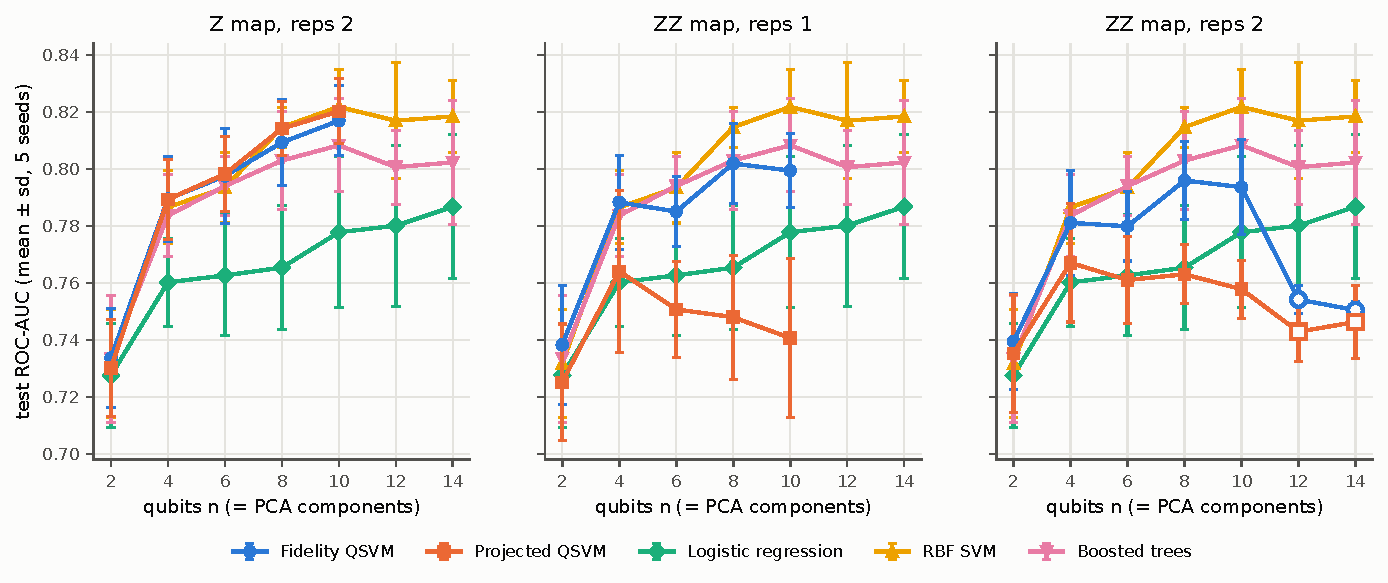
\includegraphics[width=\textwidth]{fig1_auc_vs_qubits.pdf}
\caption{Test AUC against qubit count for every model (mean $\pm$ sd over seeds), one panel per feature map. The
quantum bandwidth is chosen per seed by CV; open markers: only $c\in\{\V{bandwidths_big}\}$ searched.}
\label{fig:h1}
\end{figure}
Across all \V{nconfigs} configurations, the fidelity kernel is significantly worse than the best classical baseline in
\V{h1_fid_cb} and not significantly different in \V{h1_fid_ns}. The projected kernel is worse in \V{h1_pqk_cb} and
indistinguishable in \V{h1_pqk_ns}. Neither kernel is significantly better anywhere (\V{h1_fid_qb} of
\V{nconfigs}), and the largest mean gap is \V{h1_fid_maxgap} (fidelity) and \V{h1_pqk_maxgap} (projected).
Against the RBF-SVM alone, \V{h1_rbf_hits} configurations exceed it by more than the seed spread:
\V{h1_rbf0_desc} (\V{h1_rbf0_gap}) and \V{h1_rbf1_desc} (\V{h1_rbf1_gap}). Both are at the smallest $n$, and both lie
within the seed spread of the best classical model (\V{h1_rbf0_best}, \V{h1_rbf1_best}). About \V{h1_chance} such hits
per kernel are expected by chance under this rule. Figure~\ref{fig:h1} shows the per-seed best bandwidth. The best
classical AUC rises from \V{best_cl_n2} at $n=2$ to \V{best_cl_n10} at $n=10$. The Z map tracks it (\V{cv_z_n10_auc} at
$n=10$, gap \V{cv_z_n10_gap}). The ZZ maps fall significantly behind from $n=\V{cv_zz_first_behind}$ (gap
\V{cv_zz2_n10_gap} at $n=10$ and \V{cv_zz2_n14_gap} at $n=14$ for $r=2$). \verdict{H1 held}

\subsection{H2: geometric difference versus the AUC gap}
\begin{figure}[t]
\centering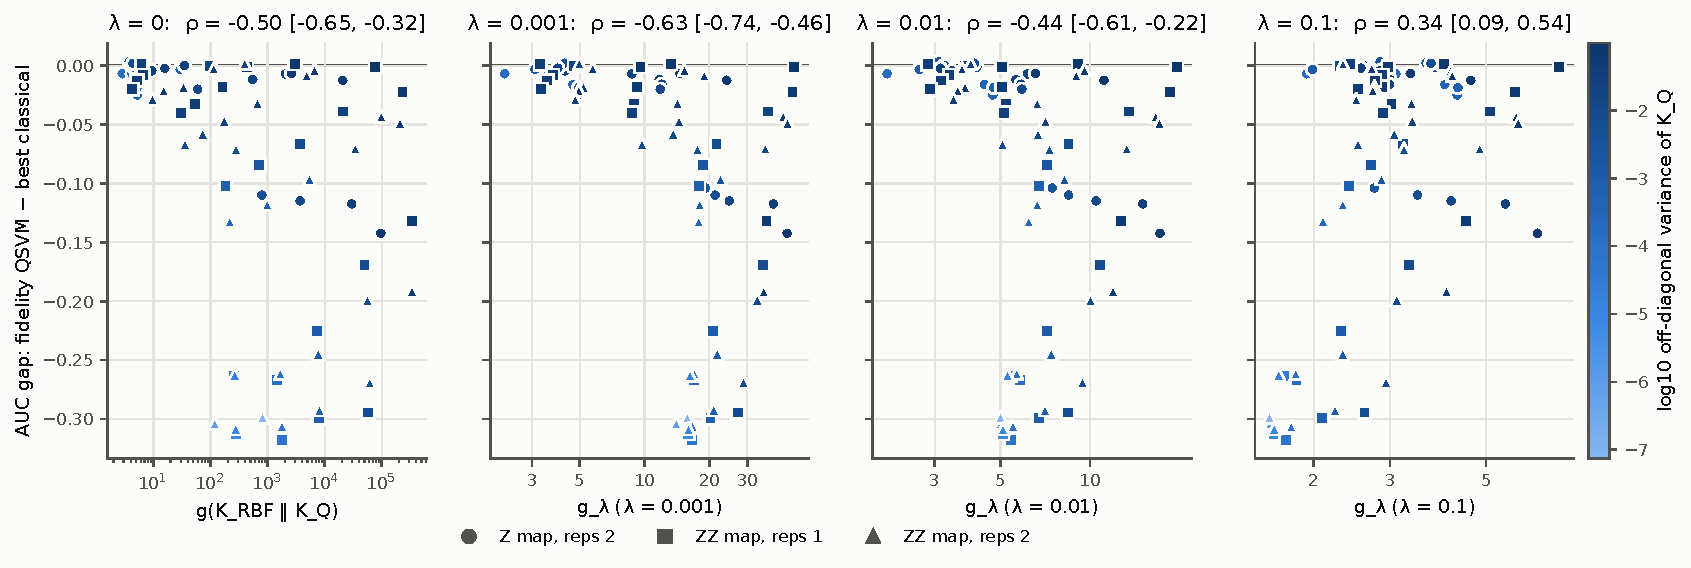
\includegraphics[width=\textwidth]{fig2_gap_vs_g.pdf}
\caption{AUC gap (fidelity kernel minus best classical) against $g$ for four $\lambda$, one point per configuration,
coloured by $\log_{10}$ off-diagonal variance; Spearman $\rho$ with 95\% bootstrap interval above each panel.}
\label{fig:h2}
\end{figure}
\begin{table}[t]
\centering\footnotesize\setlength{\tabcolsep}{3.5pt}
\caption{Spearman $\rho$ between $g$ and the AUC gap across \V{nconfigs} configurations (95\% bootstrap intervals).
H2 predicts $\rho>0$.}
\label{tab:h2}
\begin{tabular}{lcccc}
\toprule
 & $\lambda=0$ & $\lambda=0.001$ & $\lambda=0.01$ & $\lambda=0.1$\\
\midrule
pooled & \V{h2_pool_l0} & \V{h2_pool_l0001} & \V{h2_pool_l001} & \V{h2_pool_l01}\\
partial $\mid\log_{10}$ var. & \V{h2_part_l0} & \V{h2_part_l0001} & \V{h2_part_l001} & \V{h2_part_l01}\\
within Z, $r=2$ & \V{h2_within_l0_z} & \V{h2_within_l0001_z} & \V{h2_within_l001_z} & \V{h2_within_l01_z}\\
within ZZ, $r=1$ & \V{h2_within_l0_zza} & \V{h2_within_l0001_zza} & \V{h2_within_l001_zza} & \V{h2_within_l01_zza}\\
within ZZ, $r=2$ & \V{h2_within_l0_zzb} & \V{h2_within_l0001_zzb} & \V{h2_within_l001_zzb} & \V{h2_within_l01_zzb}\\
\bottomrule
\end{tabular}
\end{table}
Table~\ref{tab:h2} and Fig.~\ref{fig:h2} give the test. For the headline regularised $g$ ($\lambda=0.01$),
$\rho=\V{h2_pool_l001}$: significantly \emph{negative}. The same holds at $\lambda=0$ and $0.001$. Only $\lambda=0.1$
gives a positive pooled $\rho$ (\V{h2_pool_l01}). That correlation vanishes once concentration is controlled
(partial \V{h2_part_l01}), and within the ZZ maps the partial correlations at $\lambda=0.1$ are
\V{h2_wpart_l01_zza} and \V{h2_wpart_l01_zzb}. Kernel variance itself tracks the gap better than any $g$
($\rho=\V{h2_logvar}$). The label-aware ratio $\log_{10}(s_C/s_Q)$ is also negative ($\rho=\V{h2_ratio_pool}$; partial
\V{h2_ratio_part}). But $s_C\ge\V{h2_sc_min}$ in every configuration, so the bound $\sqrt{s}$ exceeds 1 and is vacuous.
Concentrated kernels get $s_Q$ near 1 because they memorise the labels ($\rho(s_Q,\text{AUC})=\V{h2_sq_auc}$).

\emph{Huang et al.'s necessary condition.} With $N=\V{ntrain}$, $\sqrt{N}=\V{sqrtN}$. The regularised $g$ never reaches
it: the maxima are \V{nc_max_l001} ($\lambda=0.01$) and \V{nc_max_l01} ($\lambda=0.1$), so
\V{nc_above_l001} of \V{nconfigs} configurations pass. No configuration shows an advantage, which is consistent with
the criterion. The unregularised $g$ (maximum \V{nc_max_l0}) exceeds $\sqrt{N}$ in \V{nc_above_l0} configurations.
None of them shows an advantage either (\V{nc_above_l0_cb} classical better, \V{nc_above_l0_ns} not significant); these
are mostly concentrated kernels, so passing is necessary but not sufficient. \verdict{H2 failed} $g$ does not
correlate positively with the gap.

\subsection{H3: concentration and AUC against qubit count and depth}
\begin{figure}[t]
\centering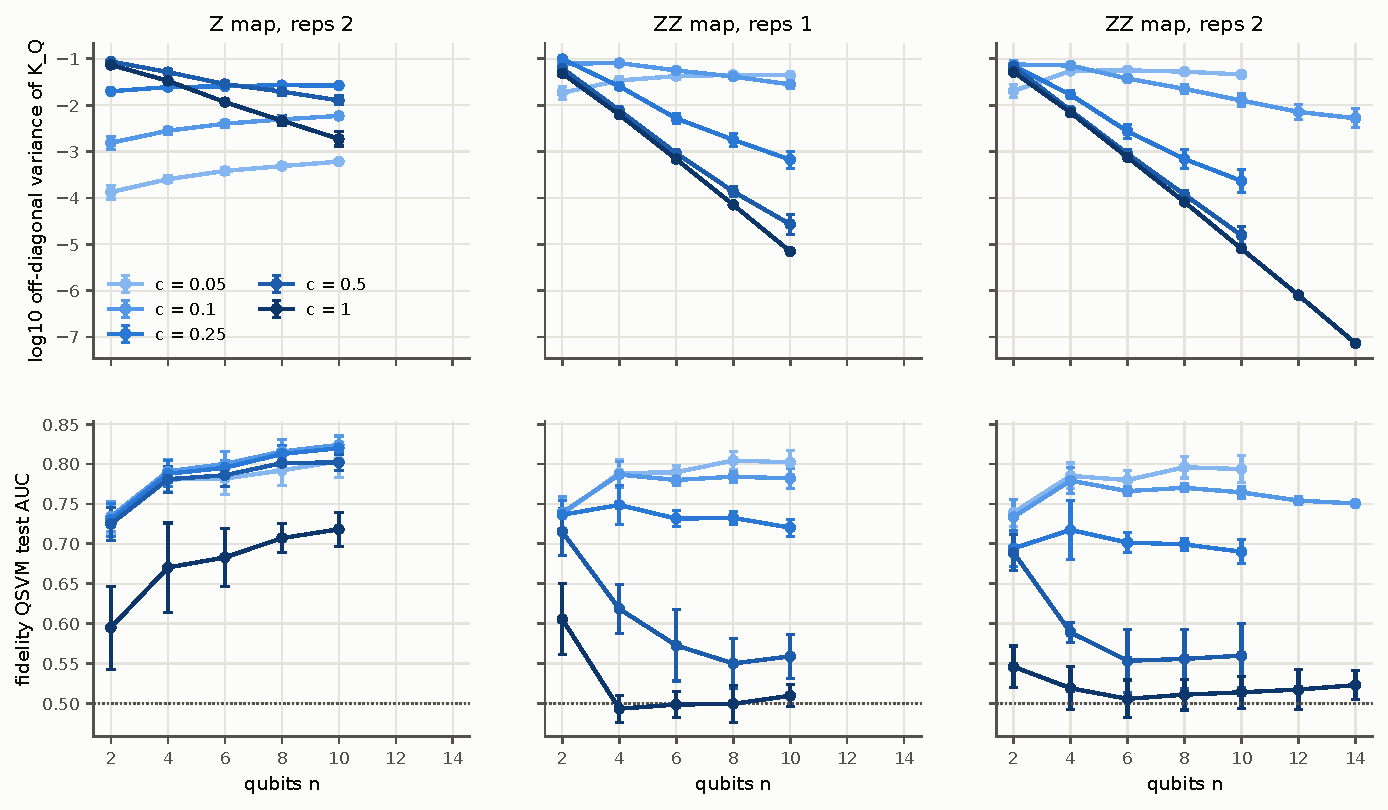
\includegraphics[width=0.85\textwidth]{fig3_concentration_vs_qubits.pdf}
\caption{$\log_{10}$ off-diagonal kernel variance (top) and fidelity-kernel AUC (bottom) against qubit count, one line
per bandwidth $c$ (mean $\pm$ sd over seeds).}
\label{fig:h3}
\end{figure}
For each feature map and bandwidth we regress $\log_{10}$ variance and AUC on $n$ (Fig.~\ref{fig:h3}). H3 requires both
to fall significantly. That happens in \V{h3_held} of \V{h3_cells} (map, $c$) cells: \V{h3_held_list}. For the ZZ maps
at $c\ge0.25$, the variance falls by \V{h3_slope_min}--\V{h3_slope_max} decades per qubit. For ZZ, $r=2$, $c=1$ it drops
from \V{ex_zz2_c1_var_n2} at $n=2$ to \V{ex_zz2_c1_var_n14} at $n=14$, while the AUC is already near chance
(\V{ex_zz2_c1_auc_n2} and \V{ex_zz2_c1_auc_n14}), so it cannot fall further. For the Z map the AUC rises with $n$ in
\V{h3_z_auc_rises} of \V{h3_z_cells} cells: more PCA components carry more information. Depth has no consistent effect.
Over \V{h3_depth_cells} matched (n, c) cells, ZZ with $r=2$ is more concentrated than $r=1$ in \V{h3_depth_more_conc}
and has lower AUC in \V{h3_depth_auc_lower}.

Low variance is not enough to predict failure. Concentrated kernels (variance $<10^{-3}$, off-diagonal mean $<0.1$;
\V{h3_conc_n} configurations) have median AUC \V{h3_conc_med} and at most \V{h3_conc_max}. Near-constant kernels
(variance $<10^{-3}$, mean $>0.5$; \V{h3_flat_n} configurations, all Z map with the smallest $c$) still reach median
AUC \V{h3_flat_med} in exact simulation. \verdict{H3 held in part} It held for the entangling map at larger
bandwidths, not for the product map or small $c$, and not for depth.

\subsection{H4: bandwidth at fixed qubit count}
\begin{figure}[t]
\centering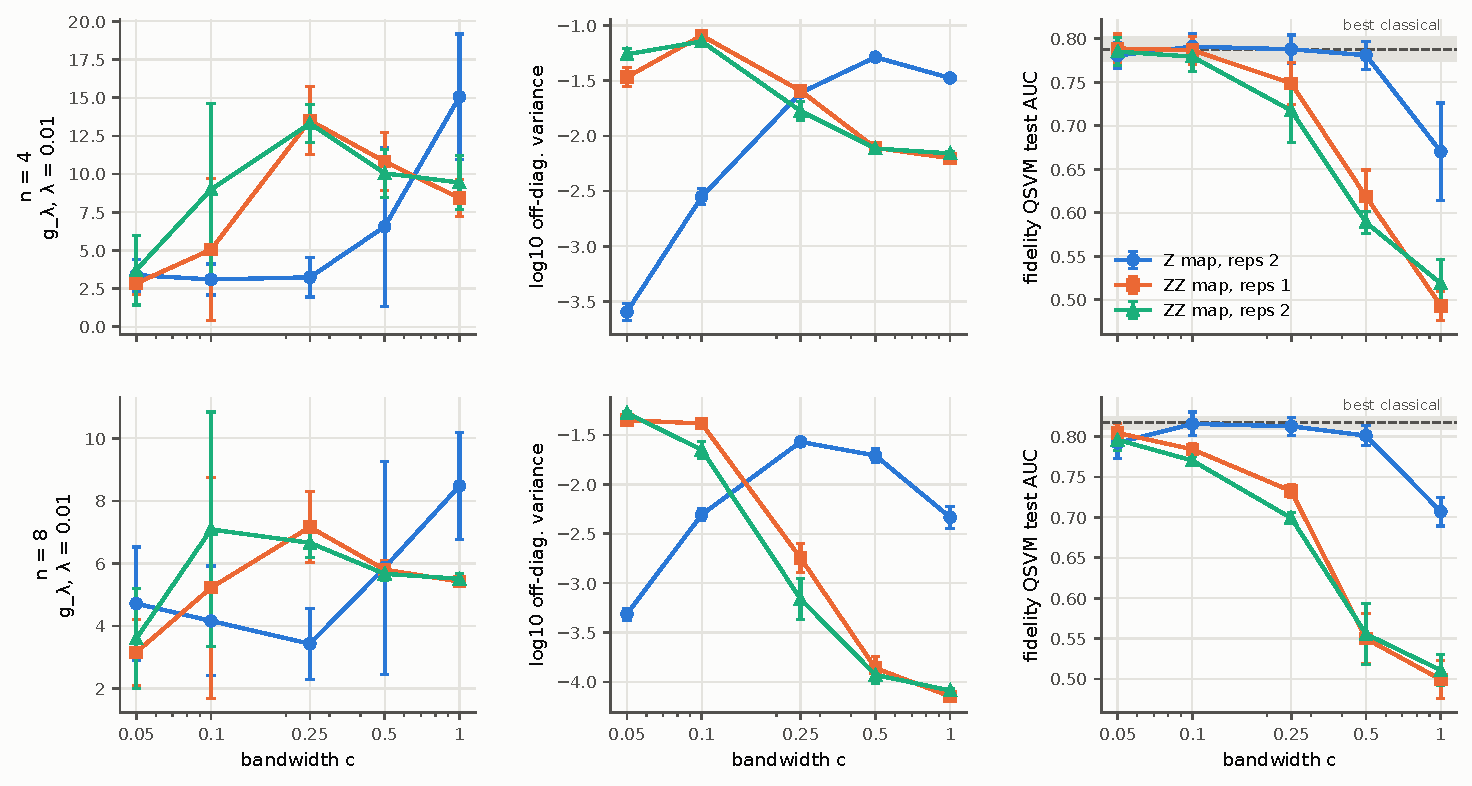
\includegraphics[width=0.85\textwidth]{fig4_vs_bandwidth.pdf}
\caption{Regularised $g$ ($\lambda=0.01$), $\log_{10}$ off-diagonal variance and fidelity-kernel AUC against bandwidth
$c$ at $n=4$ (top) and $n=8$ (bottom); the grey band is the best classical AUC $\pm$ sd.}
\label{fig:h4}
\end{figure}
In each of the \V{h4_cells} (feature map, $n$) cells of the main grid we compare $c=\V{bw_min}$ with $c=\V{bw_max}$,
paired by seed (Fig.~\ref{fig:h4}). \emph{First half.} A smaller $c$ recovers the AUC in \V{h4_auc_rec} of
\V{h4_cells} cells; for example, ZZ with $r=2$ at $n=8$ goes from \V{ex_h4_auc_large} to \V{ex_h4_auc_small}. A smaller
$c$ raises the variance (reduces concentration) in only \V{h4_var_raised} of \V{h4_cells}. In the Z-map cells and at
$n=2$, the kernel flattens towards a constant at small $c$, so its variance falls even though the AUC recovers.
\emph{Second half, and its dependence on $\lambda$.} For the headline regularised $g$ ($\lambda=0.01$), $g$ falls
steadily towards 1 as $c$ shrinks in only \V{h4_g01_mono} of \V{h4_cells} cells. For the ZZ maps it peaks at an
intermediate bandwidth ($c\in\{\V{h4_g01_argmax_zz}\}$), and at $c=\V{bw_min}$ it is still \V{h4_g01_small_min}--\V{h4_g01_small_max}.
For ZZ, $r=2$, $n=8$ it goes \V{ex_h4_g01_large} at $c=1$, maximum at $c=\V{ex_h4_g01_argmax}$, then
\V{ex_h4_g01_small} at $c=\V{bw_min}$. The unregularised $g$ ($\lambda=0$) behaves differently. It is closer to 1 at
small $c$ in \V{h4_g0_closer} of \V{h4_cells} cells and falls steadily in \V{h4_g0_mono}, from
\V{h4_g0_large_min}--\V{h4_g0_large_max} at $c=1$ to \V{h4_g0_small_min}--\V{h4_g0_small_max} at $c=\V{bw_min}$. It moves
towards 1 without getting there. \verdict{H4 held in part} The first half held for AUC and, for the ZZ maps at
$n\ge4$, for concentration. The second half failed for the regularised $g$. For the unregularised $g$ only its
direction holds.

\section{Robustness: PCA versus boosted-tree feature selection}\label{sec:robust}
\begin{figure}[t]
\centering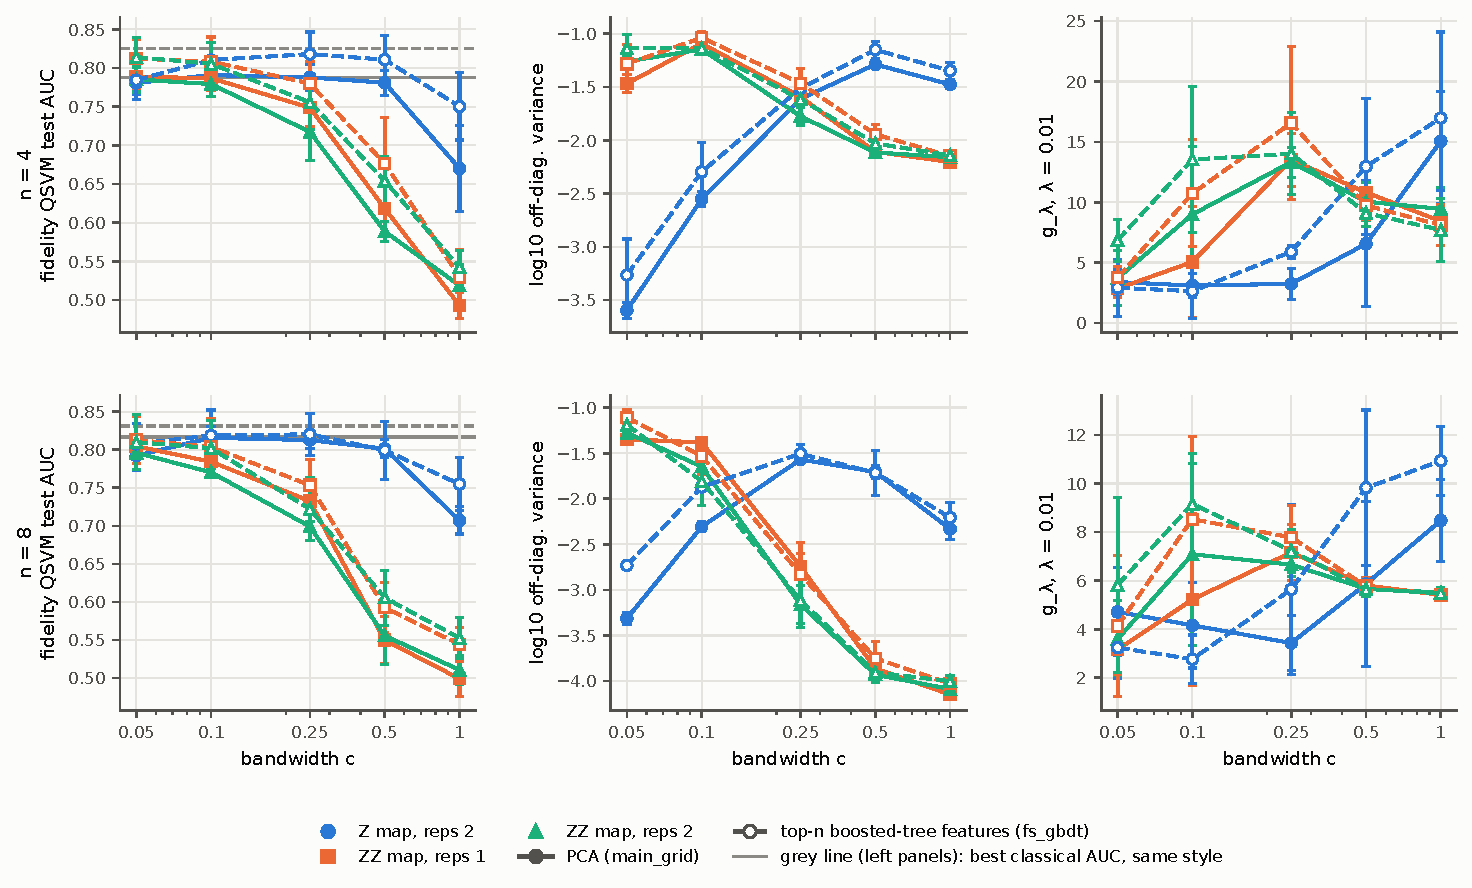
\includegraphics[width=0.85\textwidth]{fig7_robustness_feature_selection.pdf}
\caption{Fidelity-kernel AUC, $\log_{10}$ variance and $g$ ($\lambda=0.01$) against $c$ at $n=4$ and $n=8$, for PCA
(solid) and the top-$n$ boosted-tree features (dashed); grey lines are the best classical AUC.}
\label{fig:robust}
\end{figure}
We repeat the $n\in\{\V{fs_qubits}\}$ slices with the top-$n$ features by XGBoost importance, fitted on training events
only; \V{rob_top2} are always selected first. All four hypotheses are re-tested on both slices with the same code, and
\V{rob_unchanged} of 4 verdicts are unchanged (Fig.~\ref{fig:robust}).
\begin{itemize}
\item \textbf{Both sides improve.} Feature selection helps classical and quantum models alike: the best classical AUC
moves from \V{rob_bc_pca_n4} to \V{rob_bc_fs_n4} ($n=4$) and from \V{rob_bc_pca_n8} to \V{rob_bc_fs_n8} ($n=8$). The
median change over configurations is \V{rob_dbc} for the best classical and \V{rob_dq} for the fidelity kernel.
\item \textbf{H1 still holds.} No quantum kernel exceeds the best classical model (\V{rob_fs_fid_qb} and
\V{rob_fs_pqk_qb} of \V{rob_fs_nconf}). It also holds against the classical model selected by CV, stored only for these
runs (\V{rob_fs_fid_cv_qb} and \V{rob_fs_pqk_cv_qb}). Choosing the best classical model on test AUC raises it by only
\V{rob_bias} on average.
\item \textbf{H2 still fails.} $\rho$ is \V{rob_fs_h2_l001} at $\lambda=0.01$ (PCA slice: \V{rob_pca_h2_l001}) and
\V{rob_fs_h2_l0} at $\lambda=0$. The positive value at $\lambda=0.1$ (\V{rob_fs_h2_l01}) again disappears once
concentration is controlled (\V{rob_fs_h2part_l01}).
\item \textbf{H3 and H4 still hold only in part.} H3 holds in \V{rob_fs_h3_held} of \V{rob_fs_h3_cells} cells (PCA:
\V{rob_pca_h3_held}). For H4, a smaller $c$ recovers the AUC in \V{rob_fs_h4_auc} of \V{rob_fs_h4_cells} cells and
raises the variance in \V{rob_fs_h4_var}. The regularised $g$ falls steadily towards 1 in \V{rob_fs_h4_g}.
\item \textbf{Similar angle spread.} The median interquartile range of the encoded angles is
\V{ang_fs_n4}/\V{ang_fs_n8} rad with feature selection and \V{ang_pca_n4}/\V{ang_pca_n8} rad with PCA ($n=4$/$n=8$), so
the effective bandwidth is not very different.
\end{itemize}

\section{Noise study and the real-hardware run}
\begin{figure}[t]
\centering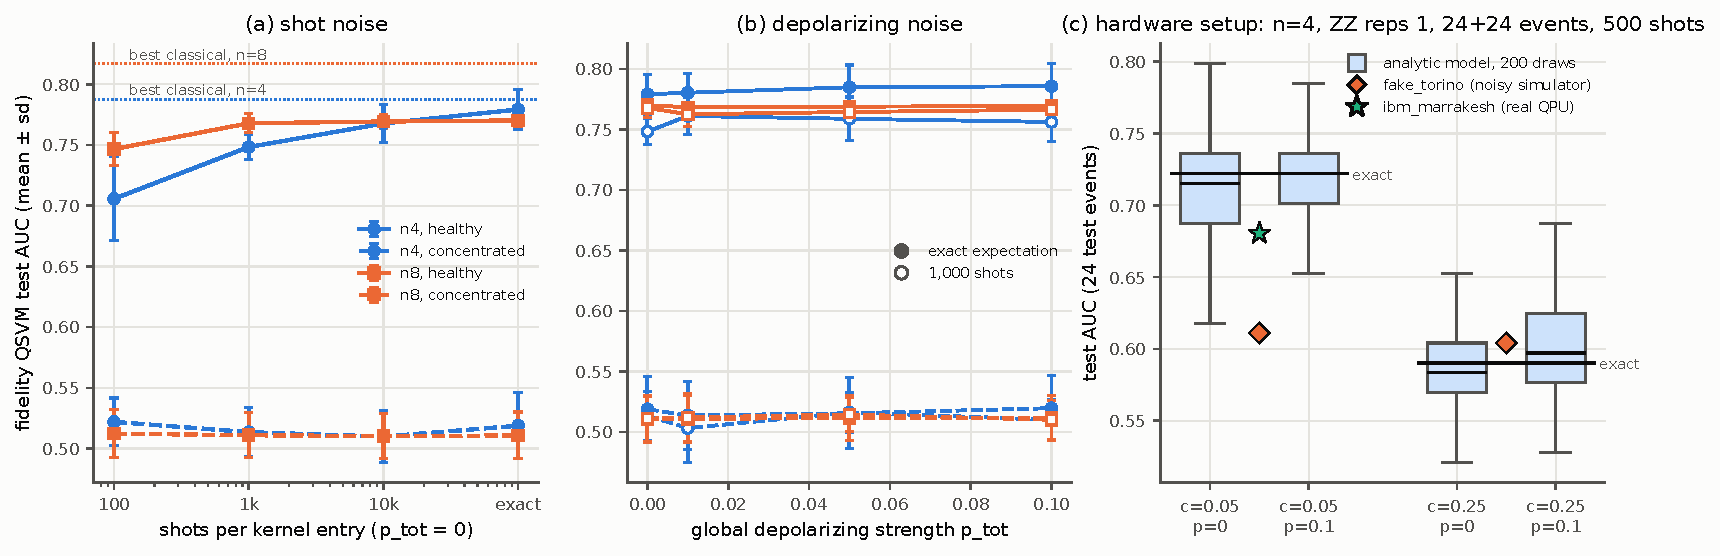
\includegraphics[width=\textwidth]{fig6_noise_and_hardware.pdf}
\caption{(a) Fidelity-kernel AUC against shots per kernel entry; (b) against global depolarising strength;
(c) the hardware setup: analytic noise model (boxes over \V{hw_draws} draws), noisy simulator and \V{hw_backend}.}
\label{fig:noise}
\end{figure}
\paragraph{Analytic noise.} We take four ZZ, $r=2$ settings: healthy ($c=\V{nz_c_healthy}$) and concentrated
($c=\V{nz_c_conc}$), each at $n=4$ and $n=8$. We re-estimate both train and test kernels with binomial shot noise
(\V{nz_shots} shots) and global depolarising noise ($p_{\rm tot}\in\{\V{nz_p}\}$), \V{nseeds} seeds each
(Fig.~\ref{fig:noise}a,b). Shot noise dominates. The healthy $n=4$ kernel goes from AUC \V{nz_h4_ex} (exact) to
\V{nz_h4_1k} (1000 shots) and \V{nz_h4_100} (100 shots). The $n=8$ kernel goes from \V{nz_h8_ex} to \V{nz_h8_100}.
Depolarising noise alone barely matters: \V{nz_h4_ex_p01} at $p_{\rm tot}=0.1$ for healthy $n=4$. The concentrated kernels
stay at \V{nz_conc_min}--\V{nz_conc_max} under every condition, against best classical AUCs of \V{nz_bc4} and \V{nz_bc8}.
Shot noise also inflates the measured variance of the concentrated $n=8$ kernel, from \V{nz_var8c_ex} to \V{nz_var8c_100}
at 100 shots. So the variance diagnostic is reliable at 1000 or more shots but can mislead at 100.

\paragraph{Hardware.} On \V{hw_backend} we ran the ZZ map with $r=\V{hw_reps}$, $n=\V{hw_n}$, $c=\V{hw_c}$, with
\V{hw_ntrain} training and \V{hw_ntest} test events and \V{hw_shots} shots. This took \V{hw_circuits} circuits (mean
depth \V{hw_depth}, \V{hw_2q} two-qubit gates) and \V{hw_qpu_s}~s of QPU time (Fig.~\ref{fig:noise}c).
\begin{itemize}
\item \textbf{Fidelity kernel:} AUC \V{hw_auc_real}, against \V{hw_auc_exact} exact and \V{hw_auc_fake} on the
\V{hw_fake_backend} noisy simulator.
\item \textbf{Projected kernel:} \V{hw_pqk_real}, against \V{hw_pqk_exact} exact and \V{hw_pqk_fake} simulated.
\item \textbf{Kernel error:} the mean absolute error of the hardware training kernel is \V{hw_mae_real}
(simulator: \V{hw_mae_fake}). Its off-diagonal mean drops from \V{hw_mean_exact} to \V{hw_mean_real}, which
corresponds to an effective global depolarising strength of \V{hw_peff_real} (simulator: \V{hw_peff_fake}).
\item \textbf{Analytic model:} at $p_{\rm tot}=0.1$ and \V{hw_shots} shots, the model gives a mean AUC of
\V{hwm_p01_mean} (5--95\%: \V{hwm_p01_q05}--\V{hwm_p01_q95}) and a kernel error of \V{hwm_p01_mae}. The hardware
AUC falls inside that range; the simulator's falls below it.
\end{itemize}
With only \V{hw_ntest} test events, these AUCs are demonstrations, not precise measurements.

\section{Discussion and limitations}\label{sec:limits}
\paragraph{What the results say about $g$.} Huang et al.\ use $g$ as a \emph{necessary condition}. A small $g$
guarantees that a classical model is competitive; a large $g$ only opens the possibility of an advantage, which must
then be confirmed with the label-aware complexities~\cite{huang2021power}. Our data are consistent with that: the
regularised $g$ never passes $\sqrt{N}$, and no configuration beats the classical baselines. What fails is the
\emph{graded} reading of $g$, in which a larger $g$ marks a more promising dataset or configuration. On these data $g$
is anti-correlated with the gap, and its only positive association disappears once kernel concentration is controlled.
Concentration explains the results better: it tracks the gap more strongly than any $g$. It accounts for the ZZ
collapse at large $c$ and $n$. It also shows two distinct low-variance regimes, a concentrated one and a near-constant
one. This matches the ``spectral degeneracy'' confound reported for power-system data~\cite{islam2026power} and the
bandwidth-to-RBF picture~\cite{slattery2023numerical,florezablan2025similarity}. A plausible reason why the
regularised $g$ does not return to 1 at small $c$ is that the small-bandwidth ZZ kernel approaches an
\emph{anisotropic} Gaussian~\cite{tekeli2026zz}, not the isotropic RBF used as $K_C$. We have not tested this.

\paragraph{Limitations.}
\begin{itemize}
\item \textbf{Simulated data and small samples.} The events are detector-level Monte Carlo, with balanced classes and
only $N=\V{ntrain}$ training events, far fewer than the classical models could use.
\item \textbf{Lenient significance.} \V{nseeds} seeds and the 1-sd rule correspond to $p\approx0.09$ per comparison,
with many comparisons. ``Not significant'' does not mean equal.
\item \textbf{Shared seeds.} All configurations reuse the same \V{nseeds} data splits, so they are not independent, and
the bootstrap intervals over configurations are optimistic.
\item \textbf{Best-of-three classical.} ``Best classical'' is selected on test AUC. This favours H1. It was measured to
be small (\V{rob_bias}), but only for the feature-selection runs.
\item \textbf{Hardware.} Only one configuration was run on hardware, with \V{hw_ntest} test events. The noise model is a
global depolarising channel, not a device model.
\item \textbf{Scope.} Only Z and ZZ maps with linear entanglement, one classical reference kernel for $g$, and a headline
$\lambda$ that is our choice, not part of the hypotheses. The hypotheses were written before the experiments but not
formally pre-registered.
\end{itemize}

\section{Conclusion and future work}
On ATLAS $H\to\tau\tau$ events, tuned classical baselines match or beat every quantum kernel we test (H1 held), so we
claim no quantum advantage. The geometric difference fails as a graded predictor of the quantum-minus-classical gap
(H2 failed). It is anti-correlated with the gap, consistent with Huang et al.'s necessary condition, and better
explained by kernel concentration. Concentration rises with qubits at fixed bandwidth for the entangling map but not
in general (H3 held in part). A smaller bandwidth recovers AUC but does not pull $g$ back towards 1 (H4 held in part).
These conclusions survive a change of feature reduction and the noise levels we studied.

Next steps follow from the literature and are cheap with the stored kernels:
\begin{itemize}
\item Kernel--target alignment as the predictor, which worked where $g$ failed on power-system data~\cite{islam2026power}.
\item $g$ against an anisotropic Gaussian reference~\cite{tekeli2026zz}.
\item Shot-noise requirements for the near-constant small-$c$ kernels~\cite{miroszewski2024shots}.
\item Larger training sets and more hardware test events.
\end{itemize}

\bibliographystyle{plainnat}
\bibliography{../docs/references}
\end{document}
